\documentclass[%
 reprint,
%superscriptaddress,
%groupedaddress,
%unsortedaddress,
%runinaddress,
%frontmatterverbose, 
%preprint,
%showpacs,preprintnumbers,
%nofootinbib,
%nobibnotes,
%bibnotes,
 amsmath,amssymb,
 aps,
%pra,
%prb,
%rmp,
%prstab,
%prstper,
%floatfix,
]{revtex4-1}

\usepackage{graphicx}% Include figure files
\usepackage{dcolumn}% Align table columns on decimal point
\usepackage{bm}% bold math
\usepackage{mathtools}
\usepackage[usenames,dvipsnames,svgnames,table]{xcolor}
\usepackage{float} %Graficos HERE
\usepackage{fancyhdr} %encabezados pro
\usepackage{braket} %notacion de dirac
\usepackage{steinmetz} %notacion fasorial
\usepackage{multirow} % filas multiples
\usepackage{cancel} %tachar terminos de ecuaciones
\usepackage{caption} 
\usepackage{subcaption} %figurasjuntas
%\usepackage{lscape} %paginas apaisadas
\usepackage{empheq} %para hacer encuadres de ecuaciones pro
\usepackage{fancybox} %encuadres chulos, junto con empheq
%\usepackage{hyperref}% add hypertext capabilities
%\usepackage[mathlines]{lineno}% Enable numbering of text and display math
%\linenumbers\relax % Commence numbering lines

%\usepackage[showframe,%Uncomment any one of the following lines to test 
%%scale=0.7, marginratio={1:1, 2:3}, ignoreall,% default settings
%%text={7in,10in},centering,
%%margin=1.5in,
%%total={6.5in,8.75in}, top=1.2in, left=0.9in, includefoot,
%%height=10in,a5paper,hmargin={3cm,0.8in},
%]{geometry}

%\preprint{APS/123-QED}
\begin{document}


\title{Feasibility Study of a CVQKD downlink}% Force line breaks with \\

\author{Marie Curie}
\author{Albert Einstein}%
\author{Richard P. Feynman}

\date{\today}% It is always \today, today,
             %  but any date may be explicitly specified

\begin{abstract}
Quantum Key Distribution (CVQKD) is one of the most important applications of Quantum Information and one that is affordable from a technological point of view. Particular interest has been put into the Continuous Variable case, because of the possibility of using entirely off-the-shelf optical components, whilst in Discrete Variable the use of single photon detectors, and often cryostats consequently, is unavoidable. Optical communication with satellites has been proposed in order to create a global QKD network. In this work we investigate and simulate the possibility of creating such a link between a ground station and a satellite, finding the probability distribution and the key rates of our CVQKD protocol, and putting exact numbers in the process that are able to reproduce a real scenario.
\end{abstract}
\maketitle
%\tableofcontents

\section{Introduction}
Quantum Key Distribution (QKD) allows the distribution of secret keys that can be used afterwards in different information processes requiring certain levels of security. Due to its theoretically unconditional security, i.e, the distribution of keys is possible whatever the computational power of a possible adversary, a lot of interest have been put into the development of this technology and its applications. 

Classically, the implementation of QKD protocols were based on discrete variables (DVQKD), and the secret information was therefore normally encoded into the polarization of photons. However, much interest is now put into the use of continuous variables instead (CVQKD), where the information is encoded in the quadratures of the quantized electromagnetic field. The main advantage of this QKD paradigm relies on the detection mechanism. While in discrete variable single photon detectors are necessary (APD or superconducting detectors), in continuous variable the detection is performed by coherent detection (homodyne or heterodyne detection), that can be implemented with off-the-shelf components working at room temperature.

The main problem of CVQKD is its tolerance to losses. The current QKD protocols can distribute keys between two points that are separated some hundreds of kilometers. If we are to create quantum networks (like the recent research on the so-called Quantum internet) we will need secure quantum and classical communication at a global scale. The transmission distance is hence the main problem of QKD protocols nowadays.

For overcoming this transmission distance problem, that is a bit more relevant in the continuous variable case, there are two proposed options. The first option is the use of quantum repeaters, where the quantum signal that is sent can be re-amplified without disturbing too much the internal quantum state of the system. Despite the interest in the developing of this technology, the current state of the art of quantum repeaters is not mature enough to have any practical implementation in the short term. To put it into perspective, the complexity of developing quantum repeaters is comparable to the complexity of building a scalable universal quantum computer.

The second option for solving the distance problem is going to space. In the vacuum of outer space, there are practically no losses and no decoherence processes either, which make it a great place for the distribution of quantum signals. The use of satellites for quantum communications is thus an active area of research.

However, the implementation of QKD in space presents several technical challenges, mainly due to the fragility of the quantum signal. The modeling of the different effects occurring in a quantum communication scenario and the study of its feasibility is crucial before launching a satellite in orbit. In this work a code was developed able to simulate a downlink quantum communication for CVQKD between a satellite and a ground station. In particular, special attention was put into the fluctuating nature of the transmission, as we will see in the next section. This fluctuations cause a different value for the key rate compared to the one that is expected from the security analysis in a static situation.



\section{Atmospheric Channel: fading}

At a given channel loss, there exists formulas that give the key rate for the prepare and measure QKD protocol. Then, in order to simulate a satellite passage, one has in principle to model the characteristics of the telescopes as well as the atmosphere, the optical and the electronic components and apply the theoretical formula that gives unconditional security. As we will see now, however, the channel transmission is not fixed at a given satellite distance, but it fluctuates. Therefore, the statistical properties of the channel should be also characterized and the key rate formula modified to take it into account in a real case scenario.

Although in space there are no losses due to interaction with matter, the beam has inevitably to cross the atmosphere, which is not trivial to model precisely because of its shifting nature, as we will see in this section.

Two atmospheric effects that are relevant for optical communication with satellites are the absorption and the scattering of light due to the different molecules and particles present in the atmosphere. They are, however, known for scientists and engineers and hence the light wavelength can be chosen so to minimize them. Their main effect at a fixed distance can be interpreted as a channel contribution to the overall loss. In a satellite passage, the distance between the satellite and the ground station changes as the satellite continues its orbit around the Earth and this losses change accordingly in a computable way.

Apart from absorption and scattering, the atmosphere presents random fluctuations in temperature due to the movement of masses of air of different sizes. Because of the relation between the index of refraction and temperature, the former is also a fluctuating quantity in the atmosphere, which in turn produce a dynamical change in the light passing through it. This is the so-called atmospheric turbulence.

Atmospheric turbulence is more critical in an uplink scenario. This is because the distribution of energy in the beam is much broader when the light arrives to the ground station from the satellite (downlink). In an uplink, however, the light is perturbed at the beginning of its path, having a potential global effect on the beam. Deflections in the direction of the beam can occur that would increase the losses in the channel even in orders of magnitude. Other effects, like scintillation and increasing of beam divergence, can also play a role due to the atmospheric turbulence. The main figure of merit describing turbulence is the so-called refractive index structure constant, $C_n^2$, that is a measure of the amount of local refractive index inhomogeneites and can then be used to quantify the strength of the optical turbulence. There exist different models for $C_n^2$ depending on location, wind speed, time of the day and year, as well as other variables. The use of one model is justified depending on the impact of turbulence in the phenomenon studied.

In fact, even in the absence of atmospheric turbulence, the measured channel transmittance has a fluctuating nature. This is mainly due to the imperfect pointing of the satellite during its orbit and to the widening of the beam waist during the light propagation.

The conclusion is then that the channel will present fluctuations, even if we consider a static scenario, where we remove the relative movement between satellite and ground station. The characterization of the pointing, divergence and turbulent effects will result in a probability distribution for the transmission coefficient, or PDTC, that will contain the statistical nature of the channel and that it's crucial for the performance of the QKD protocol in space.

\subsection{Probability Distribution in the static case}

In our analysis we focused on the downlink scenario, so that a transmitting satellite following a circular orbit with radius $H$ is sending coherent states to a ground station, equipped with a receiver telescope's aperture denoted as $a$. The distance between the center of the beam and the center of the receiving telescope is denoted by $r$. This distance fluctuates with variance $\sigma$.

In this case, the effect of turbulence is not very relevant compared to other fluctuating effects, so that we can set $C_n^2$ as a real number. This parameter will therefore be manipulable in our simulation, with values rounding the interval $10^{-13}$ to $10^{-15}\ \mathrm{m^{-2/3}}$. Under this assumption, the contribution to the variance $\sigma$ due to turbulence can be calculated as:
\begin{equation}
    \sigma_{\mathrm{turb}} = 1.919\cdot C_n^2z^3(2W_0)^{-1/3}
\end{equation}
where $z$ is the transmission distance were the atmosphere is relevant, which is taken here as an atmospheric effective height of 10 km. $W$ is the beam waist.

Apart from turbulence, the two main sources of fluctuations are due to the pointing error of the satellite, i.e. how well does the satellite track the ground station in its orbit, and the divergence error due to the fact that the beam radius is increasing as the distance from the transmitter to the receiver increases. These two loss sources can be characterized by two angles: the pointing error angle $\theta_p$ and the angle of divergence $\theta_d$. The former is defined as the angle between the line that connects the center of the telescope with the satellite and the real line. This angle will of course fluctuate causing the pointing error, and hence its name. The latter, $\theta_d$, is the plane angle formed by the end of the gaussian beam and its center due to the beam divergence.

With these definitions, the beam waist at the ground and the variance of the fluctuations due to beam wandering can be easily written as: 
\begin{equation}
    W = \theta_d\cdot h\qquad\qquad \sigma_{p}= \theta_p\cdot h
\end{equation}
where $h$ is the instantaneous distance between the satellite and the ground station.

To sum up, the beam divergence is making the footprint of the beam larger on the ground and the beam wandering is causing fluctuations in the center of the beam.

We then considered the turbulence and the beam wandering the main effects that causes fluctuations in the beam, since they are independent effects variance is:
\begin{equation}
    \sigma^2 =\sigma_p^2+\sigma_{\mathrm{turb}}^2 
\end{equation}
Following the paper by Vasylyev \textit{et al}, the transmission coefficient can be calculated from the variance $\sigma$, the aperture of the telescope, $a$, and the beam waist at the receiver, $W$. In the reference an analytic approximation is taken that differs from the numerical integration version by a small percentage, making it appropriate also for our case.

Within this approximation, the transmission coefficient can be calculated from the deflection distance $r$, as:
\begin{equation}
    T = T_0^2\exp\left(-\left(\frac{r}{R}\right)^{\lambda}\right)
    \label{T-r}
\end{equation}
where $T_0$ defines the maximum transmission coefficient, $lambda$ is called the shape parameter and $R$ the scale parameter. If we call:
\begin{equation}
 x\equiv4\left(\frac{a}{W}\right)^2
\end{equation}
then we can compute $\lambda$ and $R$ as:
\begin{equation}
\begin{split}
        \lambda = 2x\frac{e^{-x}\mathrm{I}_1(x)}{1-e^{-x}\mathrm{I}_0(x)}\left(\log \left(\frac{2T_0^2}{1-e^{-x}\mathrm{I}_0(x)}\right)\right)^{-1} \\
         R = a\left(\log\left(\frac{2T_0^2}{1-e^{-x}\mathrm{I}_0(x)}\right)\right)^{-1/\lambda}
\end{split}
\end{equation}
where $\mathrm{I}_0(x)$ and $\mathrm{I}_1(x)$ are the modified Bessel functions of the first kind evaluated at $x$.

With this, we have the explicit relation of the transmission coefficient and the distance of deflection $r$, that is a random variable. Assuming that the deviation, $\sigma$, of the random variable $r$ is gaussian distributed around a fixed distance $d$ from the center of the telescope, the distribution of the beam deflection, $r$ follows a generalized Rice Distribution. The parameters of the distribution are then variance $\sigma^2$ and offset $d$. Namely:
\begin{equation}
    P(r|\sigma, d) =\frac{r}{\sigma^2}\exp\left(\frac{-(x^2-d^2)}{2\sigma^2}\right)\mathrm{I}_0\left(\frac{rd}{\sigma^2}\right)
    \label{P-r}
\end{equation}
Given the distribution (\ref{P-r}) and the relation of $r$ and $T$, (\ref{T-r}), we obtain the probability distribution of the transmission coefficient, that we will call PDTC. The PDTC completely characterizes the fluctuations in the atmospheric channel.

It is worth to mention that it is possible to define the cumulative function $\bar{F}$, called exceedance, as the probability of having a transmission coefficient greater than a certain value $T$:
\begin{equation}
    \bar{F}(T) = \int^{\infty}_{T}\mathrm{PDTC}(\tau)\mathrm{d}\tau
\end{equation}
The exceedance has also the statistical properties of the channel and hence characterizes it completely as well. In our simulation the exceedance was calculated as a check for the normalization of the numerically computed PDTC.

In Fig. \ref{RicianDistr} we represent an example of the characterization of the channel following the above analysis for a satellite at a distance of $H=400$ km, pointing error $\theta_p=1\ \mu$rad, divergence angle $\theta_d=10\ \mu$rad, telescope aperture $a=0.75$ m, and $C_n^2=10^{-14}$ m$^{-2/3}$.

\begin{figure}
\centering
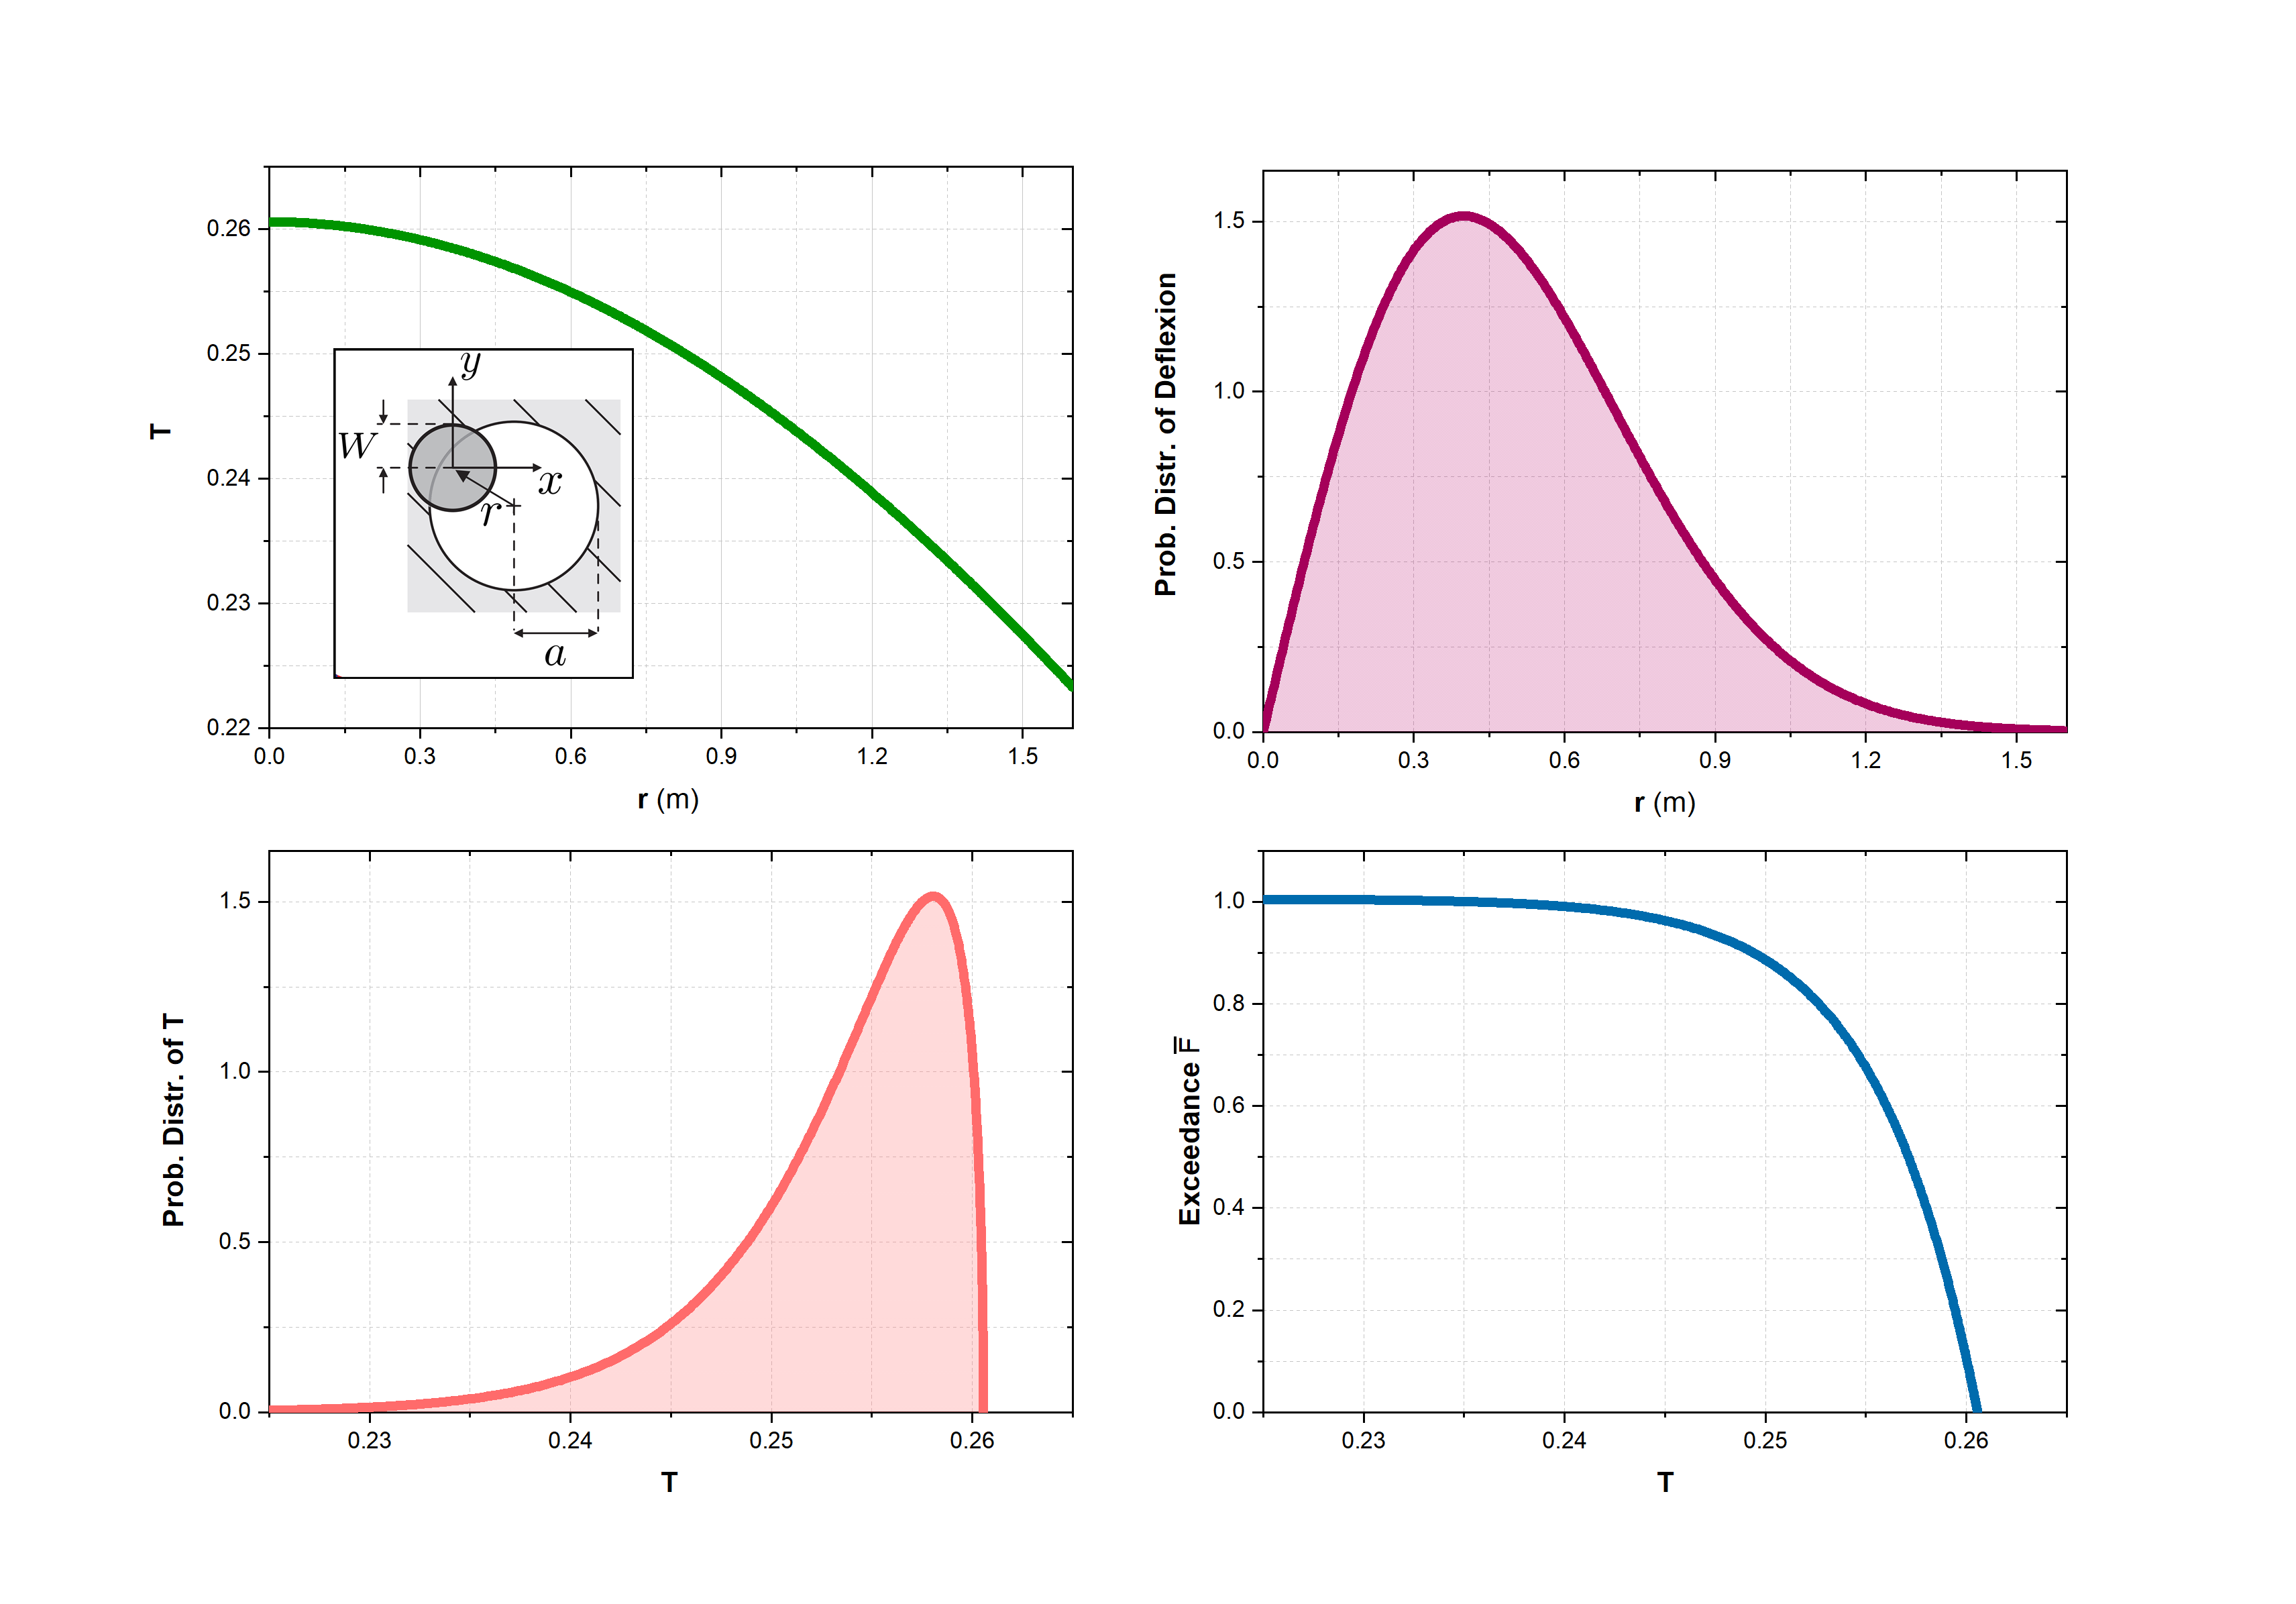
\includegraphics[width=0.5\textwidth]{RicianDistr.png}
\caption{Statistics of the atmospheric channel at a fixed distance. The relation between the transmission coefficient, $T$, and the deflection distance, $r$, together with the probability distribution of $r$, a generalized Rice Distribution, give us the probability distribution for $T$, from which the exceedance was also computed.}
\label{RicianDistr}
\end{figure}

\section{Orbit}
After the channel characterization at a fixed height $H$, the whole orbit was considered in order to obtain the probability distribution of the satellite passage.

For this purpose, a circular orbit with radius $R_T+h_s$ was considered, were $R_T$ is the Earth's radius and $h_s$ the satellite's altitude. Because of safety conditions, ground stations communicate with satellites at a maximal zenith angle of 70°, which defines the angular visibility of the satellite. The constant angular velocity of the satellite is then $\omega^2=GM_T/(R_T+h_s)^3$, where $M_T$ is the Earth's mass. From this we can deduce that the trajectory of the orbit measured from the ground station, denoted $H(t)$, would be:
\begin{equation}
    H(t)=(R_T^2+(R_T+h_s)^2-2R_T(R_T+h_s)\cos(\omega t))^{1/2}
    \label{traj}
\end{equation}
So that we know the distance of the satellite to the ground station at every moment of the passage, and viceversa: for every time step, we know the position of the satellite.

Our aim was getting the entire probability distribution of the whole passage. For this purpose the following procedure was adapted:
\renewcommand{\labelitemi}{$\blacksquare$}
 \begin{itemize}
   \item  The orbit is divided into a set of points defined by the position of the satellite at a certain time, given by the trajectory equation (\ref{traj}).
   \item For each one of these points, the Probability Distribution of the Transmission Coefficient, PDTC, is calculated as was explained in the previous section. The time difference between consecutive points is calculated as well, getting a set of numbers $\{\Delta t_i\}$.
   \item The sum of the multiplication of each $\Delta t_i$ with the corresponding PDTC computed at the point of the trajectory gives a final distribution of the time spent by the satellite with a certain transmission coefficient $T$. Indeed, if the points are close enough, the performed sum mimics an integral over the time of the orbit, namely:
   \begin{equation}
       \sum_i\mathrm{PDTC}(T,t_i)\Delta t_i\rightarrow \int \mathrm{PDTC}(T,t)\mathrm{d}t
   \end{equation}
 \end{itemize}
Fig \ref{orbits} represents three different distributions of the transmission coefficient after
The physical parameter used for the calculation of the key rate was the transmission efficiency, i.e. $\tau=T^2$. Having the PDTC in time for the whole orbit, the Probability Distribution of the transmission efficiency has then other expression, but the actual probabilities of each of them should be equal. Namely, if $\tau = \tau(T)$:
\begin{equation}
\begin{split}
     \mathrm{PDTC}(\tau(T)) = \mathrm{PDTC}(T)\frac{\mathrm{d}T}{\mathrm{d}\tau}\\
         \int_{\tau_A}^{\tau_B}\mathrm{PDTC}(\tau(T))\mathrm{d}\tau =\int_{T_A}^{T_B}\mathrm{PDTC}(T)\mathrm{d}T
    \end{split}
\end{equation}
Therefore, both distributions after the satellite passage will give us the same statistical predictions for our calculation of the key rate, and we do not need to compute explicitly the PDTE from the PDTC for every orbit.

\section{Key Rate for fading channels}
The QKD protocol used in this work was the no-switching protocol of ref () that has recently been proved secure against arbitrary attacks. In the protocol Alice samples $N$ complex numbers $\{\alpha_1,...,\alpha_N\}$ from a gaussian distribution, preparing then the coherent states $\{\ket{\alpha_1}...\ket{\alpha_N}\}$. She sends the states to Bob through the fading channel, where the transmission efficiency would change in each use of the channel in a way described by the corresponding probability distribution. Bobs performs heterodyne measurement to the states, obtaining the quadratures of the coherent states and getting $N$ complex numbers $\beta_1,...,\beta_N$.




















\end{document}
